% ============================================================
%  Data Types and Life Cycle — Learning Activity Report
%  Single-column | Overleaf-compatible (.tex)
%  Universidad Politécnica de Yucatán
% ============================================================
\documentclass[12pt, a4paper]{article}

\usepackage[T1]{fontenc}
\usepackage[utf8]{inputenc}
\usepackage{lmodern}
\usepackage[a4paper, top=2.5cm, bottom=2.5cm, left=2.5cm, right=2.5cm]{geometry}

% ── Diagrams ──────────────────────────────────────────────
\usepackage{tikz}
\usetikzlibrary{shapes.geometric, arrows.meta, positioning, calc}

% ── Tables ───────────────────────────── ───────────────────
\usepackage{booktabs}
\usepackage{array}
\usepackage{tabularx}
\usepackage{colortbl}
\usepackage{makecell}
\usepackage{multirow}

% ── Layout & style ────────────────────────────────────────
\usepackage{xcolor}
\usepackage{microtype}
\usepackage{caption}
\usepackage{fancyhdr}
\usepackage{titlesec}
\usepackage{setspace}
\usepackage{parskip}
\usepackage{hyperref}
\usepackage{abstract}
\usepackage{float}        % [H] placement — forces tables exactly here

% ============================================================
%  AQUAMARINE COLOUR PALETTE
% ============================================================
%  Pyramid / diagrams
\definecolor{aqDark}  {RGB}{0,   128, 128}   % dark teal (Wisdom)
\definecolor{aqMid}   {RGB}{64,  174, 168}   % mid aquamarine (Knowledge)
\definecolor{aqLight} {RGB}{127, 211, 205}   % light aquamarine (Information)
\definecolor{aqPale}  {RGB}{195, 238, 235}   % pale aquamarine (Data)
%  Tables
\definecolor{aqHdr}   {RGB}{0,   139, 139}   % dark cyan — header background
\definecolor{aqRow}   {RGB}{232, 250, 248}   % near-white aqua — alternating row
\definecolor{aqRule}  {RGB}{0,   128, 128}   % teal — table rule lines

% ── Page style ────────────────────────────────────────────
\pagestyle{fancy}
\fancyhf{}
\fancyhead[L]{\small\textit{Data Types and Life Cycle}}
\fancyhead[R]{\small\textit{Software Technology --- UPY}}
\fancyfoot[C]{\small\thepage}
\renewcommand{\headrulewidth}{0.5pt}
\setlength{\headheight}{14pt}

% ── Section headings — BLACK ──────────────────────────────
\titleformat{\section}
  {\normalfont\large\bfseries\color{black}}
  {\thesection.}{0.5em}{}[\vspace{-4pt}{\color{aqRule}\rule{\textwidth}{0.6pt}}]
\titleformat{\subsection}
  {\normalfont\normalsize\bfseries\color{black}}
  {\thesubsection.}{0.5em}{}
\titleformat{\subsubsection}
  {\normalfont\normalsize\bfseries\itshape\color{black}}
  {}{0em}{}
\titlespacing{\section}{0pt}{14pt}{6pt}
\titlespacing{\subsection}{0pt}{10pt}{4pt}
\titlespacing{\subsubsection}{0pt}{8pt}{3pt}

% ── Table utilities ───────────────────────────────────────
\captionsetup{font=small, labelfont=bf, skip=5pt}
\renewcommand{\arraystretch}{1.40}
\setlength{\aboverulesep}{0pt}
\setlength{\belowrulesep}{0pt}

% ── Paragraph spacing ─────────────────────────────────────
\setlength{\parindent}{0pt}
\setlength{\parskip}{6pt}

% ── Abstract style ────────────────────────────────────────
\renewcommand{\abstractnamefont}{\normalfont\normalsize\bfseries}
\renewcommand{\abstracttextfont}{\normalfont\small}
\setlength{\absleftindent}{0pt}
\setlength{\absrightindent}{0pt}

% ============================================================
%  ██  FILL IN YOUR INFORMATION — EDIT THESE LINES IN OVERLEAF  ██
% ============================================================
\newcommand{\StudentName}   {Jose Luis Rejon Quintal}   % <── STUDENT NAME
\newcommand{\MyCuatrimestre}{5th Quarter}               % <── QUARTER / TERM
\newcommand{\MyGroup}       {TSU in Data and AI}        % <── GROUP / PROGRAMME
\newcommand{\MyProfessor}   {Didier Gamboa Angulo}      % <── PROFESSOR
\newcommand{\MyDate}        {June 21, 2026}             % <── SUBMISSION DATE
\newcommand{\UniversityName}{Universidad Polit\'{e}cnica de Yucat\'{a}n} % <── UNIVERSITY
% ============================================================

% ── Helper: aquamarine table header cell ─────────────────
%  Usage: \Hcell{text}   (white bold text on aqHdr background)
\newcommand{\Hcell}[1]{{\color{white}\textbf{#1}}}

% ============================================================
\begin{document}

% ============================================================
%  COVER PAGE
% ============================================================
\thispagestyle{empty}

\begin{center}

  % ---- University block ----
  {\large\bfseries \UniversityName}\\[8pt]   %% <── CAMBIA \UniversityName arriba
  \textcolor{aqRule}{\rule{\textwidth}{1.5pt}}

  \vspace{2.5cm}

  % ---- Report title ----
  {\LARGE\bfseries Data Types and Life Cycle}\\[10pt]
  {\large Learning Activity Report}\\[6pt]
  {\normalsize Subject: Data Mining \quad\textbullet\quad Software Technology}

  \vspace{3.0cm}

  % ── STUDENT INFORMATION ──────────────────────────────────
  %  Edit the \newcommand values near the top of this file.
  %  Each command maps to one field below.
  % ─────────────────────────────────────────────────────────
  \begin{tabular}{>{\bfseries}r p{9cm}}
    Student name:    & \StudentName   \\[12pt]   %% <── edita \StudentName
    Quarter:         & \MyCuatrimestre\\[12pt]   %% <── edita \MyCuatrimestre
    Programme:       & \MyGroup       \\[12pt]   %% <── edita \MyGroup
    Professor:       & \MyProfessor   \\[12pt]   %% <── edita \MyProfessor
    Submission date: & \MyDate        \\         %% <── edita \MyDate
  \end{tabular}

  \vspace{2.5cm}

  % ---- Footer ----
  \textcolor{aqRule}{\rule{\textwidth}{0.6pt}}\\[4pt]
  {\small M\'{e}rida, Yucat\'{a}n, M\'{e}xico \quad\textbullet\quad \today}

\end{center}

\newpage

% ── TABLE OF CONTENTS ─────────────────────────────────────
\tableofcontents
\newpage

% ── ABSTRACT ──────────────────────────────────────────────
\begin{abstract}
\noindent
This report addresses four learning tasks on data concepts applied to marketing.
\textbf{Task~1} builds a DIKW pyramid illustrating how raw data evolves into
actionable wisdom through successive layers of context, interpretation, and
experience.
\textbf{Task~2} maps the data life cycle across five operational phases.
\textbf{Task~3} presents a comparative table of the four analytics levels:
descriptive, diagnostic, predictive, and prescriptive.
\textbf{Task~4} applies all preceding concepts to the Caf\'{e} Aurora loyalty
campaign, classifying data types, variable types, life cycle phases, and analytics
levels found within the case.
\end{abstract}

{\color{aqRule}\rule{\textwidth}{0.5pt}}
\vspace{6pt}

% ============================================================
\section{Task 1 --- DIKW Pyramid Applied to Marketing}
% ============================================================

The DIKW model describes the hierarchical transformation of raw data into actionable
wisdom \cite{ackoff1989}. Each level adds meaning, context, or judgment to the layer
below. Figure~\ref{fig:dikw} visualises the four levels and
Table~\ref{tab:dikw} provides definitions, marketing examples, and transitions.

% ── DIKW Pyramid (TikZ — aquamarine palette) ─────────────
\begin{figure}[ht]
\centering
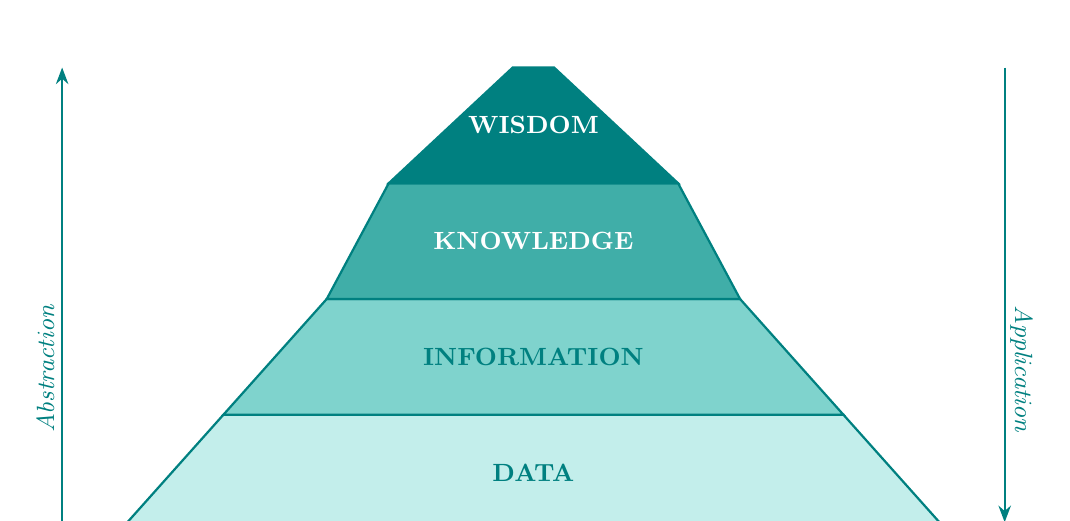
\begin{tikzpicture}[scale=1.05, font=\small]
  \def\W{5.0}    % half base width
  \def\H{1.4}    % height per level

  % ---- Level 0: DATA (bottom, lightest) ----
  \fill[aqPale]
    (-\W, 0) -- (\W, 0) --
    ({0.75*\W}, \H) -- ({-0.75*\W}, \H) -- cycle;
  \draw[thick, aqDark]
    (-\W, 0) -- (\W, 0) --
    ({0.75*\W}, \H) -- ({-0.75*\W}, \H) -- cycle;
  \node[font=\bfseries\small, text=aqDark] at (0, 0.50*\H) {DATA};

  % ---- Level 1: INFORMATION ----
  \fill[aqLight]
    ({-0.75*\W}, \H) -- ({0.75*\W}, \H) --
    ({0.50*\W}, 2*\H) -- ({-0.50*\W}, 2*\H) -- cycle;
  \draw[thick, aqDark]
    ({-0.75*\W}, \H) -- ({0.75*\W}, \H) --
    ({0.50*\W}, 2*\H) -- ({-0.50*\W}, 2*\H) -- cycle;
  \node[font=\bfseries\small, text=aqDark] at (0, 1.50*\H) {INFORMATION};

  % ---- Level 2: KNOWLEDGE ----
  % Top of this level = 0.35*\W (matches WISDOM base)
  \fill[aqMid]
    ({-0.50*\W}, 2*\H) -- ({0.50*\W}, 2*\H) --
    ({0.35*\W}, 3*\H) -- ({-0.35*\W}, 3*\H) -- cycle;
  \draw[thick, aqDark]
    ({-0.50*\W}, 2*\H) -- ({0.50*\W}, 2*\H) --
    ({0.35*\W}, 3*\H) -- ({-0.35*\W}, 3*\H) -- cycle;
  \node[font=\bfseries\small, text=white] at (0, 2.50*\H) {KNOWLEDGE};

  % ---- Level 3: WISDOM (trapezoid, wider base so text fits) ----
  % Base = 0.35*\W each side; flat apex at 0.05*\W
  \fill[aqDark]
    ({-0.35*\W}, 3*\H) -- ({0.35*\W}, 3*\H) --
    ({0.05*\W},  4*\H) -- ({-0.05*\W}, 4*\H) -- cycle;
  \draw[thick, aqDark]
    ({-0.35*\W}, 3*\H) -- ({0.35*\W}, 3*\H) --
    ({0.05*\W},  4*\H) -- ({-0.05*\W}, 4*\H) -- cycle;
  \node[font=\bfseries\small, text=white] at (0, 3.50*\H) {WISDOM};

  % ---- Side arrows ----
  \draw[-{Stealth[length=6pt]}, thick, aqDark]
    (-\W-0.7, 0.1) -- (-\W-0.7, 4*\H)
    node[midway, left, rotate=90, yshift=6pt, font=\small\itshape, text=aqDark]
    {Abstraction};
  \draw[-{Stealth[length=6pt]}, thick, aqDark]
    (\W+0.7, 4*\H) -- (\W+0.7, 0.1)
    node[midway, right, rotate=-90, yshift=6pt, font=\small\itshape, text=aqDark]
    {Application};
\end{tikzpicture}
\caption{DIKW Pyramid: from raw data to actionable wisdom.}
\label{fig:dikw}
\end{figure}

\arrayrulecolor{aqRule}
\begin{table}[ht]
\centering
\caption{DIKW Pyramid --- definitions, marketing examples, and transitions.}
\label{tab:dikw}
\small
\begin{tabularx}{\textwidth}{>{\bfseries}p{2.3cm} X X X}
\toprule
\rowcolor{aqHdr}
\Hcell{Level} &
\Hcell{Definition} &
\Hcell{Example in marketing} &
\Hcell{How it transforms to the next level} \\
\midrule
Data &
  Raw, isolated facts with no context or meaning. &
  500 customer purchases were recorded on Saturday. &
  Data is aggregated and organised to reveal patterns, becoming information. \\
\rowcolor{aqRow}
Information &
  Organised data that provides context and answers a specific question. &
  Saturday sales are 20\% higher than the weekly average. &
  Patterns in information are interpreted using experience, generating knowledge. \\
Knowledge &
  Interpreted information combined with expertise and experience. &
  Weekend customers prefer premium drinks; Friday promotions boost Saturday visits. &
  Knowledge is applied with judgment to a real situation, producing wisdom. \\
\rowcolor{aqRow}
Wisdom &
  The judicious use of knowledge to make a sound decision or take an action. &
  Launch a Friday happy-hour campaign for premium drinks to raise Saturday revenue. &
  --- \\
\bottomrule
\end{tabularx}
\end{table}
\arrayrulecolor{black}

\newpage

% ============================================================
\section{Task 2 --- Data Life Cycle}
% ============================================================

The data life cycle describes the sequential flow of data from initial collection to a
final marketing action \cite{provost2013}. Figure~\ref{fig:dlc} illustrates the five
phases with a feedback loop, and Table~\ref{tab:dlc} details each phase.

% ── Data Life Cycle Flowchart (horizontal, aquamarine) ────
\begin{figure}[ht]
\centering
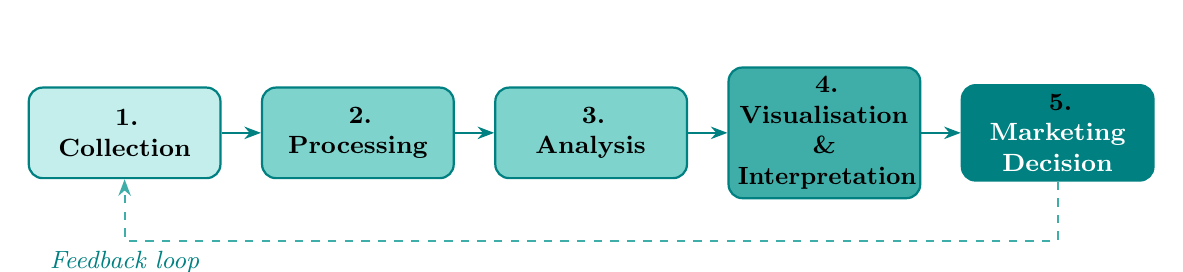
\begin{tikzpicture}[
  node distance = 0.6cm and 0.5cm,
  box/.style = {
    rectangle, rounded corners=5pt,
    minimum width=2.35cm, minimum height=1.15cm,
    text centered, font=\small\bfseries,
    draw=aqDark, thick, text width=2.2cm
  },
  arr/.style = {-{Stealth[length=6pt]}, thick, aqDark}
]
  \node[box, fill=aqPale]  (c) {1.\\Collection};
  \node[box, fill=aqLight, right=of c] (p) {2.\\Processing};
  \node[box, fill=aqLight, right=of p] (a) {3.\\Analysis};
  \node[box, fill=aqMid,   right=of a] (v) {4.\\Visualisation \&\\Interpretation};
  \node[box, fill=aqDark,  right=of v] (d) {5.\\\textcolor{white}{Marketing\\Decision}};

  \draw[arr] (c) -- (p);
  \draw[arr] (p) -- (a);
  \draw[arr] (a) -- (v);
  \draw[arr] (v) -- (d);

  % Feedback loop
  \draw[arr, dashed, aqMid]
    (d.south) -- ++(0,-0.75) -| (c.south)
    node[midway, below, font=\small\itshape, text=aqDark]
    {Feedback loop};
\end{tikzpicture}
\caption{Data Life Cycle with feedback loop.}
\label{fig:dlc}
\end{figure}

\arrayrulecolor{aqRule}
\begin{table}[ht]
\centering
\caption{Data Life Cycle --- phases, descriptions, and marketing examples.}
\label{tab:dlc}
\small
\begin{tabularx}{\textwidth}{>{\bfseries}p{2.8cm} X X}
\toprule
\rowcolor{aqHdr}
\Hcell{Phase} &
\Hcell{What occurs in that stage} &
\Hcell{Example applied in marketing} \\
\midrule
1.\ Collection &
  Raw data is gathered from primary and secondary sources such as sales
  systems, social networks, and web analytics. &
  Capturing customer transactions via POS, Instagram comments, Google Maps
  reviews, and delivery app logs. \\
\rowcolor{aqRow}
2.\ Processing &
  Data is cleaned, deduplicated, normalised, and transformed into a
  consistent, usable format. &
  Removing duplicate customer records, standardising date formats, and unifying
  channel labels (\textit{Whats / WA / WhatsApp}). \\
3.\ Analysis &
  Statistical or algorithmic methods are applied to identify patterns,
  correlations, and actionable insights. &
  Segmenting customers by purchase frequency and channel to identify
  high-value and at-risk groups. \\
\rowcolor{aqRow}
4.\ Visualisation \& Interpretation &
  Results are presented through dashboards, charts, and reports for
  decision-makers. &
  A dashboard showing sales by channel, average ticket, and satisfaction
  levels for the marketing team. \\
5.\ Marketing Decision &
  Insights are converted into concrete actions, strategies, or campaigns. &
  Allocating advertising budget to the channel with the highest repurchase
  rate and launching a loyalty promotion. \\
\bottomrule
\end{tabularx}
\end{table}
\arrayrulecolor{black}

\newpage

% ============================================================
\section{Task 3 --- Comparative Table of Analytics Levels}
% ============================================================

The four analytics levels represent progressively deeper uses of data, from
describing the past to recommending optimal future actions \cite{davenport2007}.

\arrayrulecolor{aqRule}
\begin{table}[ht]
\centering
\caption{Comparative table of analytics levels with marketing examples.}
\label{tab:analytics}
\small
\begin{tabularx}{\textwidth}{>{\bfseries}p{2.5cm} X X X}
\toprule
\rowcolor{aqHdr}
\Hcell{Analytics Level} &
\Hcell{Question it answers} &
\Hcell{What it seeks to discover} &
\Hcell{Example in marketing} \\
\midrule
Descriptive &
  \textit{What happened?} &
  Historical summaries, trends, frequencies, and distributions in past data. &
  Total units sold per product category last month, broken down by sales channel. \\
\rowcolor{aqRow}
Diagnostic &
  \textit{Why did it happen?} &
  Causes, correlations, and contributing factors behind observed outcomes. &
  Identifying that a 15\% drop in conversions coincided with a price increase
  and longer delivery times. \\
Predictive &
  \textit{What will happen?} &
  Future outcomes and probabilities estimated from historical patterns and models. &
  Forecasting that customers inactive for 45+ days have a 70\% probability of
  churning. \\
\rowcolor{aqRow}
Prescriptive &
  \textit{What should we do?} &
  Optimal actions and recommendations that maximise a desired outcome. &
  Automatically sending a personalised 10\% discount coupon to high-churn-risk
  customers. \\
\bottomrule
\end{tabularx}
\end{table}
\arrayrulecolor{black}

\newpage

% ============================================================
\section{Task 4 --- Integrative Case: Caf\'{e} Aurora}
% ============================================================

\subsection{Case Overview}

Caf\'{e} Aurora is a local coffee shop that launched a one-month loyalty campaign,
\textit{``Come Back for Your Favourite Coffee''}, targeting customers with at least
one prior purchase. Sales data were gathered from the POS system: customer name,
city, purchase date, total amount paid, number of products purchased, and purchase
channel (branch, delivery app, or WhatsApp). Social data included Instagram comments,
Google Maps reviews, and customer-posted images. Before analysis, the team corrected
inconsistent date formats, removed duplicate records, and unified channel labels
(\textit{Whats / WhatsApp / WA}). Reviews were then coded into three satisfaction
levels: low, medium, and high. Results showed that WhatsApp customers had the highest
repurchase rate, delivery customers bought fewer items per order, and negative reviews
concentrated on waiting times. Based on these findings, the coffee shop built a
dashboard and decided to strengthen WhatsApp service, improve delivery times, and
offer personalised promotions to frequent customers.

% ── Part A ───────────────────────────────────────────────
\subsubsection{Part A. Data Classification: Structured and Unstructured}

\arrayrulecolor{aqRule}
\begin{table}[H]
\centering
\caption{Classification of each data point as structured or unstructured.}
\label{tab:partA}
\small
\begin{tabularx}{\textwidth}{X p{5.5cm}}
\toprule
\rowcolor{aqHdr}
\Hcell{Data Point} &
\Hcell{Structured / Unstructured} \\
\midrule
Customer name                & Structured \\
\rowcolor{aqRow}
Customer city                & Structured \\
Purchase date                & Structured \\
\rowcolor{aqRow}
Total amount paid            & Structured \\
Number of products purchased & Structured \\
\rowcolor{aqRow}
Purchase channel             & Structured \\
Instagram comments           & Unstructured \\
\rowcolor{aqRow}
Google Maps reviews          & Unstructured \\
Images posted by customers   & Unstructured \\
\rowcolor{aqRow}
Satisfaction level           & Structured\textsuperscript{*} \\
\bottomrule
\multicolumn{2}{p{\textwidth}}{%
  \textsuperscript{*}\footnotesize
  Derived from unstructured reviews; stored as a structured ordinal variable
  (low / medium / high) after manual coding.}
\end{tabularx}
\end{table}
\arrayrulecolor{black}

% ── Part B ───────────────────────────────────────────────
\subsubsection{Part B. Variable Classification}

\arrayrulecolor{aqRule}
\begin{table}[H]
\centering
\caption{Classification of variables by statistical type.}
\label{tab:partB}
\small
\begin{tabularx}{\textwidth}{X p{5.5cm}}
\toprule
\rowcolor{aqHdr}
\Hcell{Variable} &
\Hcell{Variable Type} \\
\midrule
Customer city                & Nominal categorical \\
\rowcolor{aqRow}
Purchase date                & Date / temporal variable \\
Total amount paid            & Continuous numerical \\
\rowcolor{aqRow}
Number of products purchased & Discrete numerical \\
Purchase channel             & Nominal categorical \\
\rowcolor{aqRow}
Satisfaction level           & Ordinal categorical \\
\bottomrule
\end{tabularx}
\end{table}
\arrayrulecolor{black}

% ── Part C ───────────────────────────────────────────────
\subsubsection{Part C. Data Life Cycle in the Case}

\arrayrulecolor{aqRule}
\begin{table}[H]
\centering
\caption{Mapping of Caf\'{e} Aurora's actions to data life cycle phases.}
\label{tab:partC}
\small
\begin{tabularx}{\textwidth}{X p{4.8cm}}
\toprule
\rowcolor{aqHdr}
\Hcell{Action performed by Caf\'{e} Aurora} &
\Hcell{Life Cycle Phase} \\
\midrule
Register sales, dates, amounts, and purchase channels &
  Collection \\
\rowcolor{aqRow}
Review comments, reviews, and customer images &
  Collection \\
Correct dates with different formats &
  Processing \\
\rowcolor{aqRow}
Unify \textit{``Whats''}, \textit{``WhatsApp''}, and \textit{``WA''} into a
single category &
  Processing \\
Separate reviews into low, medium, and high satisfaction &
  Processing \\
\rowcolor{aqRow}
Identify that WhatsApp has a higher repurchase rate &
  Analysis \\
Create a dashboard with sales, satisfaction, and repurchase &
  Visualisation \& Interpretation \\
\rowcolor{aqRow}
Decide to improve delivery times and strengthen WhatsApp &
  Marketing Decision \\
\bottomrule
\end{tabularx}
\end{table}
\arrayrulecolor{black}

% ── Part D ───────────────────────────────────────────────
\subsubsection{Part D. Analytics Levels in the Case}

\arrayrulecolor{aqRule}
\begin{table}[H]
\centering
\caption{Classification of statements by analytics level.}
\label{tab:partD}
\small
\begin{tabularx}{\textwidth}{X p{2.8cm} X}
\toprule
\rowcolor{aqHdr}
\Hcell{Statement} &
\Hcell{Analytics Level} &
\Hcell{Justification} \\
\midrule
WhatsApp sales were higher than delivery sales. &
  Descriptive &
  Summarises observed sales data by channel without explaining underlying causes. \\
\rowcolor{aqRow}
Negative reviews are related to waiting times. &
  Diagnostic &
  Identifies a causal link between a service pain point (wait times) and negative
  sentiment. \\
Frequent customers might respond better to a personalised promotion. &
  Predictive &
  Projects future customer behaviour based on observed purchase frequency patterns. \\
\rowcolor{aqRow}
It is advisable to strengthen WhatsApp customer service. &
  Prescriptive &
  Recommends a specific operational action to improve an identified performance
  outcome. \\
Delivery customers buy fewer products per order. &
  Descriptive &
  Reports an observed metric (average basket size) segmented by purchase channel. \\
\rowcolor{aqRow}
It is recommended to improve delivery times. &
  Prescriptive &
  Provides a concrete, actionable recommendation derived from the diagnostic
  findings. \\
\bottomrule
\end{tabularx}
\end{table}
\arrayrulecolor{black}

\newpage

% ============================================================
\section*{Conclusions}
% ============================================================

This activity demonstrated the practical interconnection of fundamental data science
concepts. The DIKW pyramid provides a conceptual foundation for understanding how raw
facts are progressively enriched into wisdom, while the data life cycle operationalises
that transformation through five structured phases. The analytics levels framework
classifies the depth and purpose of any analytical activity, from descriptive summaries
to prescriptive recommendations. The Caf\'{e} Aurora case confirmed that even a small
business generates multiple data types---structured and unstructured---requiring careful
processing before insights can be extracted. Applying all four frameworks to a single
case revealed their interdependence: collection and processing phases align with
descriptive and diagnostic analytics, while visualisation and decision phases correspond
to predictive and prescriptive analytics. Mastering these concepts forms the analytical
foundation for data-driven marketing decision-making.

% ============================================================
%  REFERENCES
% ============================================================
\begin{thebibliography}{9}

\bibitem{ackoff1989}
  Ackoff, R.\,L. (1989).
  \textit{From data to wisdom}.
  Journal of Applied Systems Analysis, \textbf{16}, 3--9.

\bibitem{davenport2007}
  Davenport, T.\,H., \& Harris, J.\,G. (2007).
  \textit{Competing on Analytics: The New Science of Winning}.
  Harvard Business School Press.

\bibitem{provost2013}
  Provost, F., \& Fawcett, T. (2013).
  \textit{Data Science for Business: What You Need to Know about
  Data Mining and Data-Analytic Thinking}.
  O'Reilly Media.

\bibitem{rowley2007}
  Rowley, J. (2007).
  The wisdom hierarchy: representations of the DIKW hierarchy.
  \textit{Journal of Information Science}, \textbf{33}(2), 163--180.

\end{thebibliography}

\end{document}
